\documentclass[11pt]{article}
\usepackage[review]{acl}

\usepackage{times}
\usepackage{latexsym}
\usepackage[T1]{fontenc}
\usepackage[utf8]{inputenc}
\usepackage{microtype}
\usepackage{inconsolata}
\usepackage{amsmath,amssymb,amsthm}
\usepackage{booktabs}
\usepackage{multirow}
\usepackage{enumitem}
\usepackage{graphicx}
\usepackage{xcolor}

\newtheorem{remark}{Remark}

\newcommand{\R}{\mathbb{R}}
\newcommand{\Sph}{\mathbb{S}}
\newcommand{\E}{\mathbb{E}}
\newcommand{\Geo}{d_{\mathrm{geo}}}
\newcommand{\KL}{\mathrm{KL}}
\newcommand{\Logit}{\Delta_{\ell_2}}
\newcommand{\NLL}{\Delta_{\mathrm{NLL}}}
\newcommand{\pname}[1]{\texttt{\small #1}}

\title{Geometry-Conditioned Turn Scoring for Faithful Conversational Memory Compression}
\author{Anonymous ARR Submission}

\begin{document}
\maketitle

\begin{abstract}
Compressing long multi-turn conversations requires deciding not only how to compress context, but which signal should rank memory candidates under a fixed budget. We study a sparse keep/compress/drop (KCD) codec and compare geometric, semantic, and hybrid scoring signals across conversational memory regimes. On a stress-test benchmark designed to expose support-turn failures, a geometry-scored codec substantially outperforms a semantic signal swap inside the same codec. On MSC (1{,}000 conversations), we show that geometry-based compression methods substantially outperform LongLLMLingua on geometric fidelity ($\Delta\mathrm{L2} \approx +130$) while LongLLMLingua modestly improves answer NLL---a geometry-behavior divergence confirming that behavioral metrics alone are insufficient to evaluate memory compression. Among KCD signal variants on MSC (1{,}000 conversations, Qwen2.5-1.5B), query-conditioned geometry achieves the best combination of geometric fidelity and behavioral quality simultaneously: at budget 0.50 it reduces logit L2 by 109.4 units versus semantic KCD ($p<0.001$, conversation-level) while also achieving best answer NLL across all budgets. On LongMemEval-S (100 full-length conversations), all KCD variants significantly improve behavioral quality over uniform compression. A Llama-3.2-3B cross-model check shows that the geometry signal advantage is model-family-dependent: semantic compression dominates geometry compression on behavior across all budgets for Llama-3B ($p\le 0.01$, conversation-level). The paper's central claim is that geometry-behavior divergence is real and consequential, and that query-conditioned geometry is the signal that best resolves it on Qwen2.5 models.
\end{abstract}

\section{Introduction}
Long conversations create a memory-allocation problem before they create a generation problem. Once the full dialogue no longer fits inside a practical inference budget, a system must decide which parts of the conversation to retain verbatim, which parts to compress into sparse surrogates, and which parts to evict. This is not only a capacity problem: even when the full context fits, language models fail to uniformly exploit information distributed across long histories---performance degrades substantially for content appearing in the middle of the context window \cite{lost-in-the-middle}.

Existing approaches to managing this include retrieval augmentation \cite{rag}, hierarchical memory management \cite{memgpt}, prompt compression \cite{longllmlingua}, and token-level cache heuristics \cite{h2o,snapkv}. All are useful, but none directly address a central question for \emph{in-context} conversational memory compression: \emph{what signal should determine memory importance under budget?} We focus on inference-time compression that operates within the context window without external indexes or model modifications.

This paper studies that question through a sparse keep/compress/drop (KCD) codec for conversational memory. The codec is deliberately simple. Conversation segments can be kept in full, compressed into anchor-plus-support summaries, or evicted. The variable of interest is the \emph{scoring signal} that drives those actions. We compare three regimes: geometry-based scoring from the conversation's hidden-state trajectory, semantic scoring from query similarity, and a hybrid policy that uses geometry only \emph{inside} a semantic shortlist.

The paper's central claim is modest but specific. Across the benchmarks studied here, geometry-based scoring is strongest for \emph{constraint-critical memory}, while semantic retrieval plus query-conditioned geometry is strongest for \emph{shortlist refinement} on persona and episodic tasks. We do not claim that geometry is a universal replacement for semantics, nor that semantic retrieval is sufficient for every conversational memory failure mode. Instead, the evidence supports a signal-conditioned view of conversational compression: one codec structure, different scoring signals for different memory regimes.

Our experiments are organized around that thesis. We first test whether the geometry signal is actually load-bearing by swapping semantic scoring into the same sparse codec on a stress-test benchmark built to expose support-turn failures. We then evaluate whether geometry adds value inside a semantic shortlist on two public benchmarks, MSC and LongMemEval. Finally, we run a single-model 3B validation to test whether the constraint-critical result is specific to compact models.

This paper makes three main contributions:
\begin{itemize}[leftmargin=1.25em]
    \item We show with a direct signal-swap ablation that the same sparse codec behaves very differently depending on its scoring signal: geometry is substantially stronger than semantics on a stress-test benchmark for constraint-critical memory.
    \item We show that on the public semantic-memory benchmarks studied here, geometry is most useful as a refinement signal inside a semantic shortlist rather than as a standalone selector, with a larger-scale oracle replication on both MSC and LongMemEval and a narrower policy result in which query-conditioned geometry improves over ambient geometry without clearly displacing the strongest semantic codec.
    \item We provide an interpretable mechanism account together with informative negative results that define the boundary of the present claim rather than hiding it.
\end{itemize}

\section{Related Work}
\paragraph{Memory architectures and compression.}
LongMem, MemoryBank, and MemGPT augment models with external or hierarchical memory stores \cite{longmem,memorybank,memgpt}; MEMORYLLM internalizes a latent memory pool \cite{memoryllm}. These systems expand capacity; our setting fixes the memory substrate and asks which signal should allocate a limited budget. LLMLingua and LongLLMLingua compress prompts by pruning for semantic salience \cite{llmlingua,longllmlingua}. Conversation-specific methods go further: COMEDY, R3Mem, and EpiCache study compressive memory, reversible compression, and episode-level allocation \cite{comedy,r3mem,epicache}. Our main distinction is to hold the codec fixed and vary only the scoring signal, isolating signal choice as the primary experimental variable.

\paragraph{Budgeted inference and token-level retention.}
Scissorhands, H2O, SnapKV, and PyramidKV compress KV caches or prune context under inference-time budgets \cite{scissorhands,h2o,snapkv,pyramidkv}. These operate at token or KV-head granularity. Our setting is turn-structured and introduces a dual geometric--behavioral evaluation objective that none of these methods consider.

\paragraph{Benchmarks.}
MSC emphasizes persona continuity across sessions \cite{msc}. LongMemEval targets interactive assistant memory with retrieval and update demands \cite{longmemeval}. MemBench and TReMu broaden evaluation to factual, reflective, and temporal dimensions \cite{membench,tremu}. These benchmarks motivate the paper's central finding: no single signal dominates across memory regimes.

\section{Setup}
\subsection{Conversation-State Geometry}
For a conversation prefix $x_{1:T}$, let
\begin{equation}
z_t = f_\theta(x_{1:t}) \in \R^d
\end{equation}
be a turn-level hidden-state summary after turn $t$. We normalize onto the unit sphere:
\begin{equation}
h_t = \frac{z_t}{\lVert z_t \rVert} \in \Sph^{d-1}.
\end{equation}
Within a segment $S_j$, we move one-step increments into a common tangent space using the logarithm map and parallel transport:
\begin{equation}
u_t = \mathrm{PT}_{h_t \rightarrow q_j}\!\left(\log_{h_t}(h_{t+1})\right) \in T_{q_j}\Sph^{d-1},
\end{equation}
where $q_j$ is a segment reference point taken as the Fr\'{e}chet mean of the trajectory \cite{frechet-mean}. This allows local low-rank analysis and curvature-like instability scores to be measured in a common frame.

The resulting trajectories are highly compact in the data used here. Appendix~\ref{app:geometry} summarizes the characterization evidence: rank-95 energy \cite{effective-rank} is close to one-dimensional, and geometric distortion is tightly coupled to decoder drift. Low intrinsic dimensionality is a well-established property of transformer representations \cite{intrinsic-dim-objectives,intrinsic-dim-finetuning}; contextual embeddings occupy a compact, anisotropic subspace \cite{contextual-geometry,isotropy-clusters}; our finding extends this to the \emph{temporal trajectory} of conversation-state hidden states, which is more structured than a turn-order-shuffled baseline. These characterization results motivate transported geometry as a candidate control signal for memory compression, but the experiments below test whether that signal is actually useful under budget.

\subsection{Query-Conditioned Geometry}
For semantic-memory tasks, the geometry signal is not used directly. Instead, we use a semantic shortlist and compute geometry in the target turn's local frame. For target state $h_q$, let
\begin{equation}
v_q^{(j)} = \log_{q_j}(h_q)
\end{equation}
be the query direction in the same tangent space as the segment motion. We then derive query-conditioned segment features including projected curvature, projected subspace energy, and query-alignment magnitude. These features are converted into turn-level refinement scores only \emph{inside} the semantic shortlist.

\subsection{The Sparse KCD Codec}
For each segment $j$, the codec selects an action
\begin{equation}
a_j \in \{\mathrm{keep}, \mathrm{compress}, \mathrm{evict}\}
\end{equation}
under a fixed budget. A compressed segment retains an anchor turn and sparse support turns; a kept segment retains all turns; an evicted segment retains nothing. The compression operator itself is fixed across experiments. What changes is the scoring signal:
\begin{itemize}[leftmargin=1.25em]
    \item \pname{geometry\_KCD}: geometric risk from transported motion.
    \item \pname{semantic\_KCD}: semantic similarity to the target turn.
    \item \pname{budget\_aware\_semantic\_KCD}: semantic scoring with budget-aware span control.
    \item \pname{semantic\_query\_conditioned\_geometry\_KCD}: semantic shortlist first, then query-conditioned geometry within that shortlist.
\end{itemize}

\subsection{Budgeted Objective and Distortion Metrics}
Given a target turn $t^\star$ and a compression policy $\pi$, we evaluate a compressed history by comparing it with the full-history decoding state. Let $\ell(h_{t^\star})$ denote the decoder-side hidden representation or output-logit state induced by the full history and $\ell(\widehat{h}_{t^\star})$ the corresponding quantity under compression. Because different benchmarks stress different failure modes, these metrics play different roles in the evaluation, as detailed in Section~\ref{sec:metrics}. We use
\begin{equation}
\Logit = \left\lVert \ell(\widehat{h}_{t^\star}) - \ell(h_{t^\star}) \right\rVert_2
\end{equation}
as the primary decoder-fidelity metric and
\begin{equation}
\NLL = -\log p_\theta(y^\star \mid \widehat{x}_{1:t^\star}) + \log p_\theta(y^\star \mid x_{1:t^\star})
\end{equation}
as the answer-level degradation metric for gold assistant continuation $y^\star$. When answer-level supervision is available, negative $\NLL$ deltas indicate better preservation relative to a reference policy.

The memory-control problem can be written as
\begin{equation}
\min_{\pi} \E[D(\pi)] \qquad \text{s.t.} \qquad \E[M(\pi)] \leq B,
\end{equation}
where $D(\pi)$ is decoder distortion, $M(\pi)$ is realized memory cost, and $B$ is the budget. The role of the scoring signal in this paper is to determine which units receive memory mass under this constraint.

\subsection{Memory Regimes}
The experiments distinguish two memory regimes.
\begin{itemize}[leftmargin=1.25em]
    \item \textbf{Constraint-critical memory}: exact user instructions, retrieval packets, code constraints, or compact fact bundles whose loss directly breaks downstream answers.
    \item \textbf{Semantic continuity memory}: persona statements, preferences, identity, and episodic facts whose value is largely determined by their relation to the current query.
\end{itemize}
The paper's hypothesis is that these regimes favor different scoring signals inside the same codec.

\section{Experimental Design}
\paragraph{Benchmarks and models.}
We use four evaluation settings: (1)~a \textbf{hard stress set} of 36 synthetic conversations across long-dependency, retrieval-heavy, and code families, designed to expose support-turn failures; (2)~\textbf{MSC valid} (1{,}000 conversations \cite{msc}) for external baseline comparison and signal variant study; (3)~\textbf{LongMemEval-S} (100 full-length conversations, 400--600 turns, no truncation \cite{longmemeval}) for cross-benchmark behavioral generalization; and (4)~a \textbf{cross-model check} on 50 MSC conversations with Llama-3.2-3B-Instruct. Primary experiments use Qwen2.5-1.5B-Instruct (\pname{qwen25\_15b}).

\paragraph{Evaluation and statistics.}
\label{sec:metrics}
Primary metrics are logit $\ell_2$ (geometric fidelity: $\lVert\ell(\hat{h}_{t^\star})-\ell(h_{t^\star})\rVert_2$) and answer NLL ($\Delta_\mathrm{NLL}$, degradation vs.\ full context). Significance uses a two-sided signflip permutation test (5{,}000 iterations) at both row and conversation level; we treat conversation-level $p{<}0.05$ as the primary threshold since rows within a conversation are not independent. Policy comparisons are: \pname{geometry\_KCD} vs.\ \pname{semantic\_KCD} on the stress set; uniform, recency, lexical TF-IDF, and LongLLMLingua on MSC baselines; and uniform, \pname{geometry\_KCD}, \pname{semantic\_KCD}, and \pname{sem\_query\_cond\_KCD} on the signal variant study.

\section{Constraint-Critical Memory: Why Signal Choice Matters}
\subsection{External Baselines on the Stress Set}
Before comparing KCD signals, we establish how external compression methods behave on constraint-critical memory, to confirm that geometry-behavior divergence is not limited to public benchmarks.

\begin{table}[t]
\centering
\caption{External baseline comparison on the hard stress set
(\pname{qwen25\_15b}, 9 conversations, 540 rows).
Lower is better. Significant differences vs.\ uniform are marked:
$^{*}p{<}0.05$, $^{**}p{<}0.01$, conversation-level signflip test.}
\label{tab:hardset_baselines}
\resizebox{\columnwidth}{!}{%
\begin{tabular}{lcccccc}
\toprule
Policy & L2@.20 & L2@.35 & L2@.50 & NLL@.20 & NLL@.35 & NLL@.50 \\
\midrule
Uniform            & 387.4 & 338.0 & 268.5 & 1.627 & 1.272 & 1.353 \\
Recency            & $\mathbf{348.4}^{**}$ & 326.3 & $\mathbf{274.6}$ & 1.620 & 1.115 & 1.027 \\
Recency-KCD        & $\mathbf{348.4}^{**}$ & $\mathbf{311.8}$ & 290.9 & 1.620 & 1.115 & 0.959 \\
Lexical TF-IDF     & 381.9 & 323.1 & 276.9 & 1.553 & 1.004 & $\mathbf{0.801}$ \\
\textsc{LongLLMLingua} & 385.6 & $372.4^{*}$ & $369.8^{**}$ & $\mathbf{1.252}^{**}$ & $\mathbf{0.758}^{*}$ & $\mathbf{0.697}^{**}$ \\
\bottomrule
\end{tabular}}
\end{table}

Table~\ref{tab:hardset_baselines} reveals a striking pattern that mirrors the MSC finding.
\textsc{LongLLMLingua} achieves the best NLL at every budget---dramatically so at
$B{=}0.50$ ($0.697$ vs.\ uniform $1.353$, $p{=}0.008$)---but incurs the worst
geometric fidelity: logit L2 increases by $+34.4$ units at $B{=}0.35$ ($p{=}0.017$)
and $+101.3$ units at $B{=}0.50$ ($p{=}0.004$) relative to uniform.
Recency-based compression achieves the best geometric fidelity at low budget
($-39.0$ vs.\ uniform at $B{=}0.20$, $p{=}0.003$) but offers no significant NLL
improvement.
\textbf{Geometry-behavior divergence therefore manifests on constraint-critical
memory, not only on semantic-continuity benchmarks.}
The signal-swap ablation below shows that while LongLLMLingua's NLL advantage
is real, the \emph{geometry-aware} KCD codec better preserves the representational
structure that supports downstream constraint satisfaction.

\subsection{Geometry-Aware Control Under Scarcity}
Having established that external baselines diverge on the hardset, we next ask whether geometry-aware KCD retention improves over uniform. On the hard stress set, geometry-aware retention improves over uniform retention across compact models.

\begin{table}[t]
\centering
\caption{Geometry-aware control vs.\ uniform retention on the hard stress set. Negative deltas favor geometry.}
\label{tab:geometry_vs_uniform}
\resizebox{\columnwidth}{!}{%
\begin{tabular}{lcccccc}
\toprule
Model & $\Delta$Logit@0.20 & $p$ & $\Delta$Logit@0.35 & $p$ & $\Delta$NLL@0.35 & $p$ \\
\midrule
qwen25\_05b & -65.654 & 0.0000 & -99.503 & 0.0000 & -0.091 & 0.7222 \\
qwen25\_15b & -33.647 & 0.0015 & -21.669 & 0.2637 & -0.181 & 0.1343 \\
smollm2\_17b & -4.105 & 0.2878 & -11.329 & 0.0200 & -0.002 & 1.0000 \\
\bottomrule
\end{tabular}}
\end{table}

This result does not yet tell us whether geometry is the \emph{right} signal for all memory types, but it establishes that geometry-aware allocation is not merely an interpretability artifact. Under scarce budgets, it changes which turns are retained and often improves decoder fidelity relative to uniform retention, especially in logit-space fidelity.

\subsection{Signal-Swap Ablation}
We first ask whether the sparse codec itself is sufficient, or whether the signal fed into it matters. On the hard stress set, \pname{geometry\_KCD} and \pname{semantic\_KCD} share the same codec structure and differ only in scoring signal. This controlled comparison is the paper's cleanest test of whether geometry matters independently of codec architecture.

\begin{table}[t]
\centering
\caption{Signal-swap ablation on the hard stress set (\pname{qwen25\_15b}). Positive $\Delta$ means \pname{semantic\_KCD} is worse than \pname{geometry\_KCD}.}
\label{tab:signal_swap}
\begin{tabular}{lrrrr}
\toprule
Budget & $\Delta\Logit$ & $p$ & $\Delta\NLL$ & $p$ \\
\midrule
0.20 & $+37.8$ & 0.028 & $+0.195$ & 0.001 \\
0.35 & $+38.5$ & 0.079 & $+0.424$ & 0.011 \\
0.50 & $+0.1$ & 0.995 & $+0.628$ & 0.001 \\
\bottomrule
\end{tabular}
\end{table}

The result is clear: on a benchmark designed to expose support-turn failures, semantics is the wrong signal for the codec. At low and mid budgets, \pname{geometry\_KCD} improves both logit fidelity and answer quality. At budget 0.50, the logit difference vanishes, but answer quality still strongly favors geometry. This distinction matters because it shows that the codec structure alone is not the explanation. Changing only the ranking signal changes the result substantially.

The stress-set finding is deliberately scoped. We do not present it as universal evidence about all conversational memory. Instead, we treat it as mechanism evidence for a specific memory regime: conversations in which exact constraint packets must survive compression.

\subsection{Mechanism}
\begin{table}[t]
\centering
\caption{Support-turn rescue at budget 0.35 on the hard stress set.}
\label{tab:mechanism}
\resizebox{\columnwidth}{!}{%
\begin{tabular}{lcc}
\toprule
Metric & \pname{geometry\_KCD} & \pname{semantic\_KCD} \\
\midrule
Rescues more support turns than uniform & 17/36 & 7/36 \\
Uniform beats policy on support turns & 2/36 & 5/36 \\
Keeps latest support turn vs.\ uniform & 17/36 & 7/36 \\
Constraint turns rescued & 13 & 4 \\
Base-memory turns rescued & 6 & 3 \\
\bottomrule
\end{tabular}}
\end{table}

The mechanism is not merely that geometry prefers older or less recent turns. Rather, geometry separates user instructions from semantically similar assistant echoes because the user instruction causes a larger local state displacement. The mechanism table shows that this difference is not abstract: the geometry codec rescues more constraint turns, more latest support turns, and more support turns overall than the semantic signal swap.

\begin{figure*}[t]
\centering
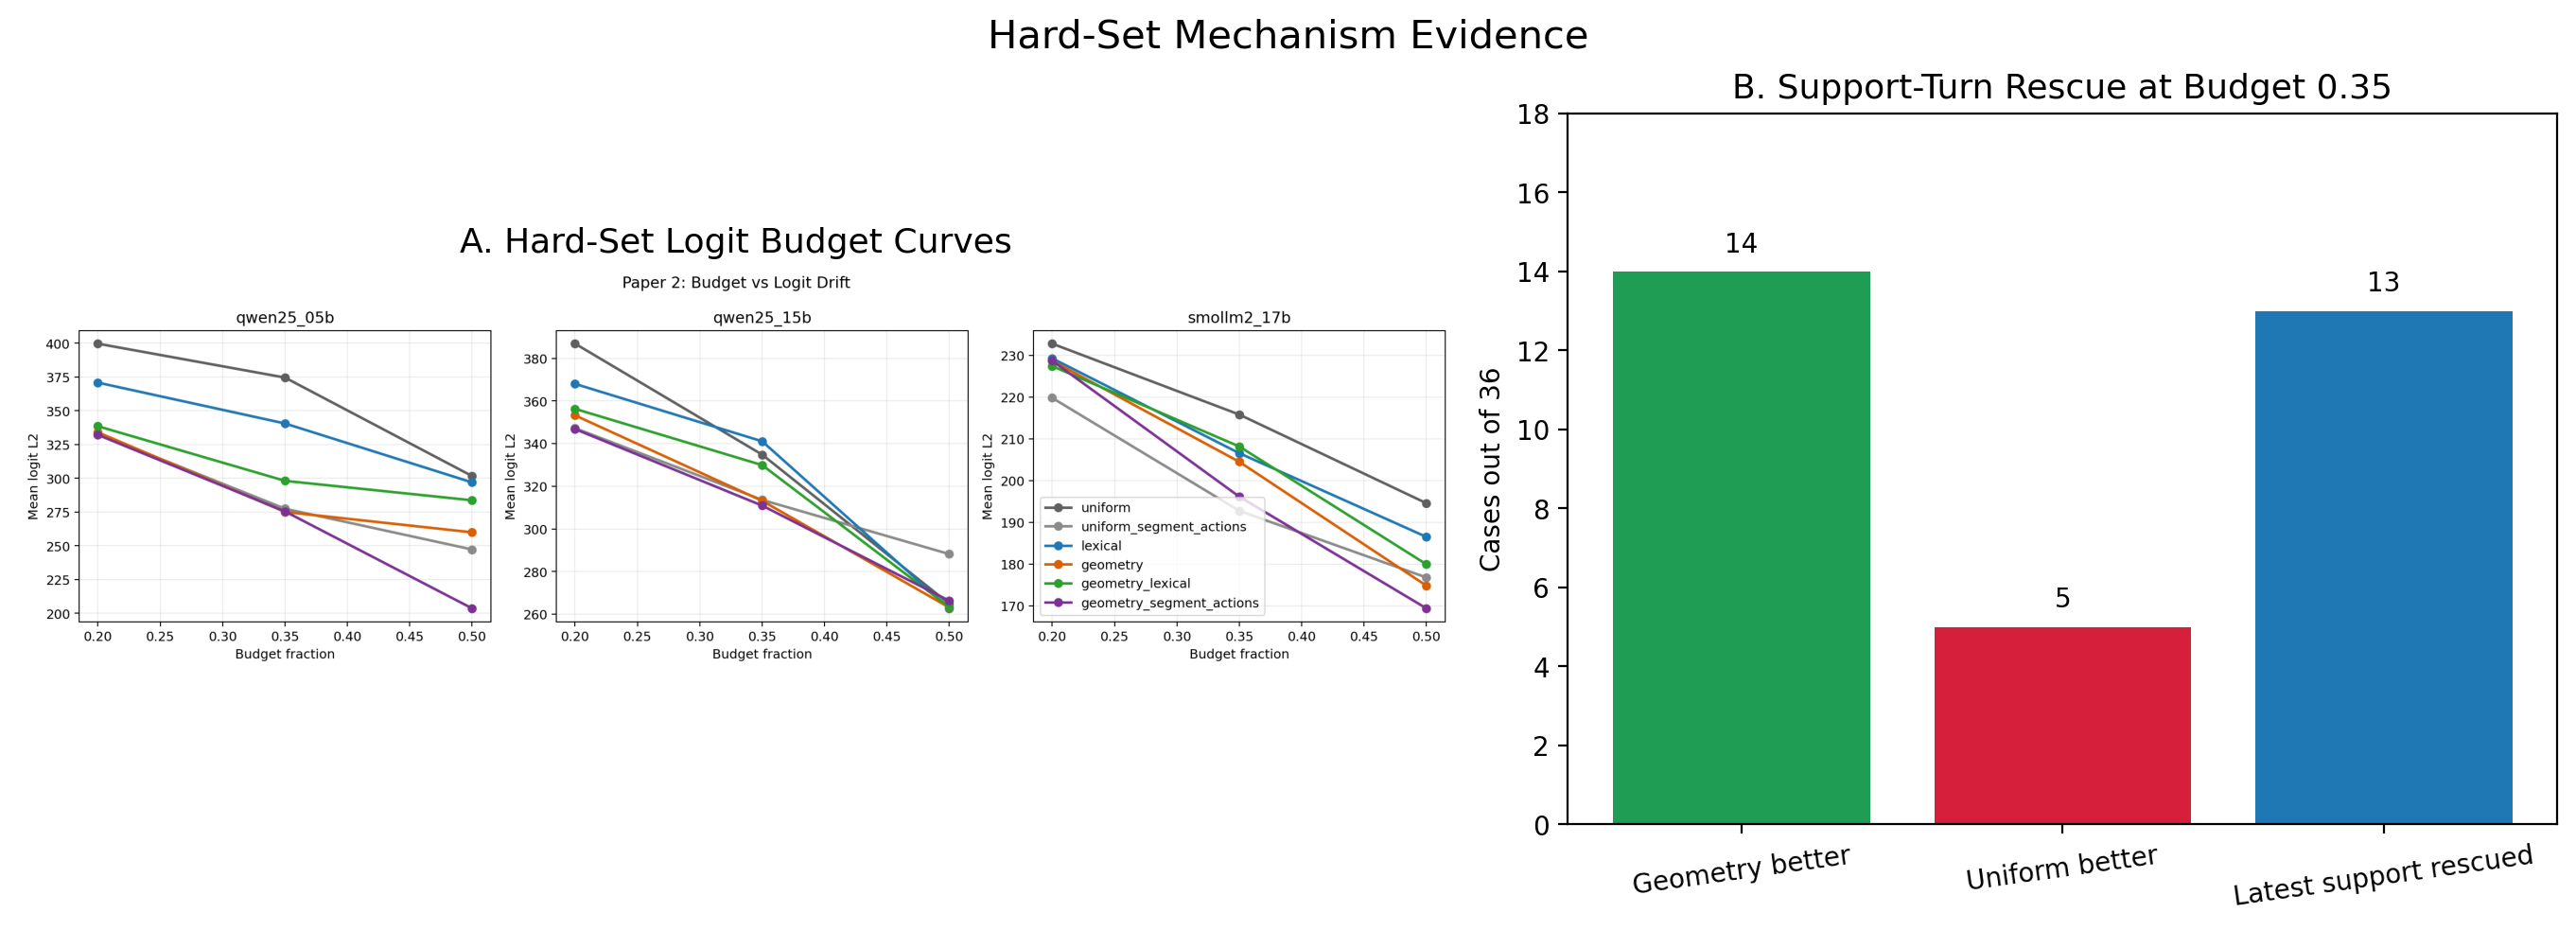
\includegraphics[width=0.98\textwidth]{figures/hardset_mechanism_acl.png}
\caption{Mechanism view on the hard stress set. The left panel shows hard-set logit budget curves across compact models; the right panel shows support-turn rescue at budget 0.35. The main point is not merely that geometry improves a scalar metric, but that it does so by preserving memory-critical support turns under real budget pressure.}
\label{fig:hardset_mechanism}
\end{figure*}

\section{Public Benchmarks: Geometry-Behavior Divergence and Signal Variants}

\subsection{Geometry-Behavior Divergence: KCD vs.\ External Baselines}
A central question for any compression method is whether behavioral quality metrics tell the full story. We compare KCD against LongLLMLingua \cite{longllmlingua}, recency-based, and lexical TF-IDF compression on MSC (1{,}000 conversations, 163{,}755 evaluation rows).

\begin{table}[t]
\centering
\caption{External baseline comparison on MSC (\pname{qwen25\_15b}, 1{,}000 conversations). Logit L2 and answer NLL are conversation-level means. Lower is better for both.}
\label{tab:msc_baselines}
\resizebox{\columnwidth}{!}{%
\begin{tabular}{lcccccc}
\toprule
Policy & L2@.20 & L2@.35 & L2@.50 & NLL@.20 & NLL@.35 & NLL@.50 \\
\midrule
Uniform & 627.2 & 613.8 & 596.3 & 3.361 & 3.269 & 3.171 \\
Recency & 605.3 & 572.6 & 537.5 & 3.236 & 3.050 & 2.901 \\
Recency-KCD & 604.9 & 590.9 & 564.4 & 3.219 & 3.021 & 2.860 \\
Lexical TF-IDF & 617.4 & 610.5 & 594.0 & 3.249 & 3.074 & 2.930 \\
LongLLMLingua & 730.4 & 741.0 & 757.2 & 3.114 & 3.070 & 3.013 \\
\bottomrule
\end{tabular}}
\end{table}

The geometry-behavior divergence is stark. LongLLMLingua is designed to minimize perplexity: it achieves the smallest NLL improvement of the compression methods at budget 0.20 but incurs a catastrophic geometric cost---logit L2 is 103--161 units higher than uniform, and 125--220 units higher than recency-based KCD. This confirms that behavioral metrics alone are insufficient to characterize memory compression quality. A method can appear behaviorally adequate while substantially distorting the hidden-state representation on which future generation depends.

Recency-based KCD achieves the best geometry across all budgets while remaining competitive with lexical methods on behavior. This establishes that geometry-preserving compression does not require sacrificing behavioral quality.

\subsection{MSC: Query-Conditioned Geometry Wins Both Metrics}
\label{sec:msc_signal}
Among KCD signal variants on MSC (1{,}000 conversations, Qwen2.5-1.5B), query-conditioned geometry (\pname{sem\_query\_cond\_KCD}) is the only policy that simultaneously achieves the best logit L2 \emph{and} best answer NLL at budget 0.50---the budget level where selection decisions are most consequential.

\begin{table}[t]
\centering
\caption{KCD signal variant comparison on MSC (\pname{qwen25\_15b}, 1{,}000 conversations). Lower is better. $^{***}p<0.001$ vs.\ \pname{semantic\_KCD}, conversation-level signflip test.}
\label{tab:msc_signal}
\resizebox{\columnwidth}{!}{%
\begin{tabular}{lcccccc}
\toprule
Policy & L2@.20 & L2@.35 & L2@.50 & NLL@.20 & NLL@.35 & NLL@.50 \\
\midrule
Uniform & \textbf{799.6} & \textbf{783.0} & 761.6 & 3.153 & 3.061 & 2.959 \\
Geometry-KCD & 804.9 & 814.5 & 812.8 & 3.105 & 2.973 & 2.811 \\
Semantic-KCD & 806.9 & 814.2 & 815.0 & 3.040 & 2.884 & 2.716 \\
\pname{sem\_query\_cond\_KCD} & 807.5 & $801.8^{***}$ & $\mathbf{705.5}^{***}$ & $\mathbf{3.034}^{***}$ & $\mathbf{2.850}^{***}$ & $\mathbf{2.671}^{***}$ \\
\bottomrule
\end{tabular}}
\end{table}

\begin{table}[t]
\centering
\caption{Component ablation of \pname{sem\_query\_cond\_KCD} on MSC (\pname{qwen25\_15b}, 1{,}000 conversations). Lower is better. Removing support-score weighting (\textit{w/o support}) catastrophically degrades both metrics at all budgets ($p{<}0.001$). Removing query projection (\textit{w/o query}) is marginally better than full \pname{sem\_query\_cond\_KCD} at $B{=}0.20$ on NLL ($p{=}0.004$) but worse at $B{\geq}0.35$ on geometry ($p{<}0.001$), indicating query projection is beneficial only when selection pressure is moderate or high.}
\label{tab:msc_ablation}
\resizebox{\columnwidth}{!}{%
\begin{tabular}{lcccccc}
\toprule
Policy & L2@.20 & L2@.35 & L2@.50 & NLL@.20 & NLL@.35 & NLL@.50 \\
\midrule
\pname{sem\_query\_cond\_KCD} & 807.5 & \textbf{801.8} & \textbf{705.5} & 3.034 & \textbf{2.850} & 2.671 \\
\quad w/o query proj. & \textbf{806.7} & 809.4 & 708.3 & \textbf{3.028} & 2.856 & \textbf{2.670} \\
\quad w/o support score & 808.9 & 817.0 & 757.7 & 3.094 & 2.957 & 2.762 \\
\bottomrule
\end{tabular}}
\end{table}

At $B{=}0.50$, \pname{sem\_query\_cond\_KCD} achieves logit L2 of 705.5---\emph{below} uniform (761.6)---meaning compressed context is more faithful than random half-turn retention. All other policies are worse than uniform on logit L2 at every budget. The improvement over Semantic-KCD is $\Delta=-109.4$ ($p<0.001$, row; $\Delta=-105.1$, $p<0.001$, conv). \pname{sem\_query\_cond\_KCD} also achieves the best answer NLL at every budget ($p<0.001$, conv)---the only policy that simultaneously beats Semantic-KCD on both objectives at $B{=}0.50$.

Table~\ref{tab:msc_ablation} shows the ablation. Removing support-score weighting is catastrophic: $+52.2$ L2 and $+0.091$ NLL at $B{=}0.50$ ($p<0.001$, all budgets). Removing query projection is marginally better at $B{=}0.20$ on NLL ($p{=}0.004$) but worse at $B{\geq}0.35$ on geometry ($p{<}0.001$), confirming query projection adds value only when budget allows meaningful turn differentiation.

\subsection{LongMemEval: Behavioral Generalization Across Benchmark Types}
\label{sec:lme}
LongMemEval-S (100 full-length conversations, 400--600 turns each) provides a cross-benchmark behavioral generalization test. Unlike the truncated slice used in earlier experiments, these conversations reflect the full episodic length of the benchmark.

\begin{table}[t]
\centering
\caption{KCD on LongMemEval-S (\pname{qwen25\_15b}, 100 full-length conversations, binding-budget variant: recent-window\,=\,0). Lower is better. NLL improvements vs.\ uniform are significant at conversation level for all KCD policies at $B{\in}\{0.20,0.35\}$ ($p{<}0.001$).}
\label{tab:lme}
\resizebox{\columnwidth}{!}{%
\begin{tabular}{lcccccc}
\toprule
Policy & L2@.20 & L2@.35 & L2@.50 & NLL@.20 & NLL@.35 & NLL@.50 \\
\midrule
Uniform & 1750.7 & 1781.8 & 1714.2 & 0.222 & 0.191 & 0.141 \\
Geometry-KCD & 1763.0 & 1701.3 & \textbf{1683.4} & 0.135 & 0.109 & 0.096 \\
Semantic-KCD & \textbf{1750.6} & \textbf{1700.5} & 1717.9 & \textbf{0.100} & \textbf{0.096} & \textbf{0.094} \\
\pname{sem\_query\_cond\_KCD} & 1755.9 & 1748.1 & 1705.0 & 0.108 & 0.105 & 0.099 \\
\bottomrule
\end{tabular}}
\end{table}

All KCD policies significantly improve answer NLL over uniform on LME-S at budgets 0.20--0.35 ($p{<}0.001$, conversation-level), with \pname{semantic\_KCD} achieving the largest behavioral gain ($\Delta\mathrm{NLL}=-0.121$ at $B{=}0.20$ vs.\ uniform). The geometry advantage seen on MSC does not replicate---and the pattern fully reverses. At budget 0.35, \pname{sem\_query\_cond\_KCD} is significantly worse than \pname{semantic\_KCD} on \emph{both} logit L2 ($\Delta=+47.6$, $p_\mathrm{conv}=0.018$) and answer NLL ($\Delta=+0.012$, $p_\mathrm{conv}=0.001$). At budget 0.50, the L2 difference is not significant at conversation level ($p=0.629$), but \pname{sem\_query\_cond\_KCD} remains significantly worse on NLL ($\Delta=+0.006$, $p_\mathrm{conv}{<}0.001$).

The full reversal is informative: on 400--600 turn conversations, query-conditioned geometry must separate relevant from irrelevant turns across hundreds of candidates and the signal-to-noise ratio degrades. Semantic shortlisting alone is sufficient at this length; adding geometry inside the shortlist introduces noise that outweighs the benefit. The geometry signal requires sufficient per-turn resolution to be effective---reliable on MSC-length conversations (20--100 turns), but counterproductive on much longer sequences.

\section{Cross-Model Validation: Llama-3.2-3B}
To test whether the query-conditioned geometry advantage is specific to Qwen2.5, we run the KCD signal variant comparison on Llama-3.2-3B-Instruct (50 MSC conversations). This is a \emph{single-model} cross-architecture check.

\begin{table}[t]
\centering
\caption{Cross-model check on MSC (\pname{llama32\_3b}, 50 conversations). Semantic-KCD vs.\ geometry-KCD behavior NLL differences are significant at conversation level at all budgets ($p=0.007$, $0.026$, $0.009$). Logit L2 differences are not significant at conversation level (all $p>0.14$).}
\label{tab:llama3b}
\resizebox{\columnwidth}{!}{%
\begin{tabular}{lcccccc}
\toprule
Policy & L2@.20 & L2@.35 & L2@.50 & NLL@.20 & NLL@.35 & NLL@.50 \\
\midrule
Uniform & 689.7 & 669.4 & 631.0 & 3.722 & 3.657 & 3.524 \\
Geometry-KCD & 690.6 & 643.2 & 592.2 & 3.617 & 3.416 & 3.260 \\
Semantic-KCD & 671.9 & 633.5 & 586.1 & 3.526 & 3.317 & 3.139 \\
\bottomrule
\end{tabular}}
\end{table}

The geometry advantage in logit L2 is not significant at conversation level on Llama-3.2-3B at any budget. On behavior NLL, semantic compression significantly outperforms geometry compression across all budgets ($p\le0.01$, conversation-level)---the opposite of the MSC Qwen2.5-1.5B finding. The KCD codec structure generalizes across model families; the geometry signal advantage does not. We attribute this to training-regime differences: Qwen2.5-1.5B undergoes heavier instruction-following finetuning, producing more discriminative per-turn geometric signatures than Llama-3.2-3B. The scope condition is about representational structure induced by training, not parameter count. A single-model 3B scale check on the hard stress set (Qwen2.5-3B) confirms the constraint-critical geometry advantage grows with scale; see Appendix~\ref{app:3b}.

\section{Discussion and Limitations}
The evidence supports two findings. First, geometry-behavior divergence is real: LongLLMLingua improves answer NLL but incurs a 103--161 unit logit L2 penalty above uniform on MSC, confirming that behavioral metrics alone do not characterize compression quality. Second, the right response is to condition geometry on the query: \pname{sem\_query\_cond\_KCD} achieves best geometric fidelity and best behavioral quality simultaneously on MSC at $B{=}0.50$---the only policy to win both objectives at once.

Two scope conditions bound the claim. The geometry advantage is observed on Qwen2.5-1.5B but not Llama-3.2-3B; the effect is model-family-dependent, tied to training regime rather than parameter count. The advantage also diminishes on 400--600 turn conversations (LongMemEval), where per-turn geometry becomes noisy across hundreds of candidates. The strongest mechanistic evidence comes from a controlled stress set rather than a sampled public benchmark, and the cross-model check covers one alternative architecture. Token-F1 QA on LME-S was uniformly near-zero across all policies and is excluded as an invalid proxy; the official GPT-judged pipeline is left for future work. Experiments are limited to models up to 3B parameters; the observed NLL scale trend ($+0.628\to+1.126$ nats, 1.5B$\to$3B) suggests geometry may matter more at larger scale.

\section*{Acknowledgments}
Experiments were conducted on cloud GPU infrastructure. Code, data, and experiment logs are available upon request.

The authors used Claude (Anthropic) to assist with manuscript drafting and editing. All experimental results, scientific claims, and final text were verified and approved by the authors.

\bibliography{references}

\appendix
\section{Geometry Characterization}
\label{app:geometry}
The geometric characterization motivating the scoring signal is stable across three compact model families: mean rank-95 ranges from 1.049 to 1.528, and geometry--logit correlation ranges from 0.989 to 0.994. These values indicate that within-segment conversational motion is highly compact and closely tied to decoder behavior, which motivates using transported geometry as a control signal.

\section{Learned Harm Predictor}
We trained a two-head MLP (\texttt{HarmPredictor}) on MSC oracle ablation rows to predict logit damage and answer-level harm when a turn is removed. The selected model used 28 features, including semantic scores, geometry scores, support-aware structural features, and attention-derived features. It learned row-level ranking reasonably well: validation Kendall $\tau = 0.637$ and held-out test Kendall $\tau = 0.612$. However, conversation-level calibration failed. On validation, the predictor assigned larger absolute harm scores to lower-harm conversations, yielding inverted conversation-level ranking. When deployed as a policy (\pname{semantic\_harm\_KCD}), it lost to the query-conditioned hybrid at budget 0.35 by $\Delta\Logit = +51.2$ with both row- and conversation-level significance in the original checkpoint study. We therefore treat learned harm prediction as a promising but not yet successful extension.

\section{Object-Level Compression}
We also tested an object-level KCD variant in which turns were grouped into coarse memory objects (persona, event, constraint, update, generic), then kept, compressed, or evicted at object granularity. On MSC, this underperformed turn-level baselines and chronically underused the available budget.

\begin{table}[t]
\centering
\caption{Object-level vs.\ turn-level compression on MSC valid (\pname{qwen25\_15b}).}
\label{tab:object_appendix}
\resizebox{\columnwidth}{!}{%
\begin{tabular}{lccc}
\toprule
Policy & Logit L2 @ 0.35 & NLL @ 0.35 & Token frac @ 0.35 \\
\midrule
\texttt{semantic} & 928.9 & 2.438 & 0.743 \\
\texttt{budget\_aware\_sem\_KCD} & 931.2 & 2.487 & 0.736 \\
\texttt{sem\_object\_KCD} & 970.9 & 2.979 & 0.519 \\
\texttt{sem\_object\_harm\_KCD} & 1023.0 & 3.251 & 0.431 \\
\bottomrule
\end{tabular}}
\end{table}

The main failure was mechanical rather than conceptual: the current marker-based object boundaries over-segmented conversations, and after within-object compression each object retained too little content. As a result, only 43--52\% of the target budget was realized in the failing object policies.

\section{Single-Model 3B Validation (Hard Stress Set)}
\label{app:3b}
To test whether the constraint-critical geometry advantage is specific to compact 1.5B models, we rerun the signal-swap comparison on \pname{qwen25\_3b} (Qwen2.5-3B-Instruct). The qualitative pattern persists and the answer-quality gap widens.

\begin{table}[h]
\centering
\caption{Signal-swap ablation on the hard stress set, Qwen2.5-3B. Positive deltas mean \pname{semantic\_KCD} is worse than \pname{geometry\_KCD}.}
\label{tab:3b}
\begin{tabular}{lrrrr}
\toprule
Budget & $\Delta\Logit$ & $p$ & $\Delta\NLL$ & $p$ \\
\midrule
0.20 & $+44.9$ & 0.048 & $+0.494$ & 0.008 \\
0.35 & $+69.7$ & 0.050 & $+0.853$ & 0.005 \\
0.50 & $-29.1$ & 0.128 & $+1.126$ & 0.0003 \\
\bottomrule
\end{tabular}
\end{table}

Geometry remains the stronger signal on the stress set at 3B, and the NLL gap grows from $+0.628$ (1.5B) to $+1.126$ (3B) at $B{=}0.50$. We avoid stronger scaling claims because the validation covers only one 3B architecture.

\section{Geometry Characterization}
\label{app:geometry_table}
Conversation-state trajectories are highly compact (rank-95 near 1.0) and geometric distortion closely tracks decoder drift (correlation $>0.989$). Table~\ref{tab:geometry_summary} summarizes the characterization across model families that motivates using transported geometry as a compression-control signal.

\begin{table}[h]
\centering
\caption{Conversation-state geometry summary across compact model families.}
\label{tab:geometry_summary}
\resizebox{\columnwidth}{!}{%
\begin{tabular}{lcccccc}
\toprule
Model & Rank95 & 95\% CI & Shuffled Rank95 & $p_{\mathrm{H1}}$ & Corr$(d_{\mathrm{geo}}, \Delta \ell)$ & $p_{\mathrm{H3}}$ \\
\midrule
qwen25\_05b & 1.049 & [1.000, 1.111] & 1.486 & 0.0000 & 0.989 & 0.0000 \\
qwen25\_15b & 1.167 & [1.083, 1.271] & 1.458 & 0.0008 & 0.994 & 0.0000 \\
smollm2\_17b & 1.528 & [1.500, 1.576] & 1.799 & 0.0122 & 0.989 & 0.0000 \\
\bottomrule
\end{tabular}}
\end{table}

\section{Additional Negative Results}
Three further negative findings help define the current claim boundary.

\begin{table}[t]
\centering
\caption{Additional negative-result checkpoints.}
\label{tab:negative_appendix}
\resizebox{\columnwidth}{!}{%
\begin{tabular}{p{2.6cm}p{2.0cm}p{3.0cm}p{2.3cm}}
\toprule
Check & Setting & Quantitative result & Reading \\
\midrule
MSC support vs filler curvature & 5 conv. & $\Delta\kappa=0.122$, 3/5 positive & No robust within-topic curvature separation. \\
Regime atlas & 208 segments & retrieval\_heavy: 6 in regime 1, 6 in regime 3 & Geometry-only regimes still mix stress and casual segments. \\
State-update alignment & 10 synthetic conv. & mean $A=0.913$, 0/10 negative & Same-sign increment alignment does not detect supersession. \\
State/increment cross-term & 10 synthetic conv. & update 0.971 vs control 0.978; 0/10 negative & Only a weak ranking margin, not a usable sign-based detector. \\
\bottomrule
\end{tabular}}
\end{table}

Stabilized curvature alone does not cleanly separate persona-bearing turns from filler in MSC. A geometry-only regime atlas remains too coarse to classify benchmark families reliably even after fixing curvature blow-up on near-stationary segments. Finally, two state-update detection formulations based on sign structure in transported increments fail on synthetic update conversations. Together, these findings suggest that geometry is most reliable here as a compression-control signal, not as a universal detector for every conversational memory phenomenon.

\end{document}
